\chapter{Scoping}

\section{Introduction}

The deliverable should consist of a library that simplifies the development of distributed client-server applications based upon a concept of room. Videogames largely use rooms in every feature (match, lobby, trading room etc.) but there are lots of potential different domains where such idea can be applied (chatrooms, for instance).
\\
The main idea of the product is to provide a low level support that handles all aspects of communication, so that developers that use the library can focus on program logic itself, without concerning about issues due to networking, serialization, synchronization between clients, integration of clients and rooms, and so on.
\\
Hence, the library provides three main notions of:
\begin{itemize}
\item \textbf{Room}: place where clients can gather to do something.
\item \textbf{Server}: a game server where rooms can be hosted.
\item \textbf{Client}: entity that might do operation on rooms, such as joining, sending messages etc.
\end{itemize} 

\section{System Requirements}

\subsection{Room}

A room is something that clients can join and interact with.
\\
Rooms have a type and are distinguishable by an univocal id.
\\
A room possesses a behavior and a state that embed the custom logic of the game. Obviously those vary from room to room, so the developer will be able to flexibly define its own type of room, namely a room that possesses its own state and behavior.

\bigskip
Rooms can be public or private. A public room can be joined by everyone; on the contrary, private rooms need a specific password to be joined.
Public rooms can be created by clients and server both, while private rooms can be set up just by clients.  
\\
It must be possible to make a public room private, and so to set a password in such room. Similarly, a private room could be made public, and the existing password must be deleted so the room can be freely joined.  

\bigskip
Rooms must expose a locking feature that permits to lock/unlock them. While locked, the room can not be joined by any new client. By default room are unlocked.
Server should have the possibility to lock/unlock a given room.

\bigskip
Rooms closing can be automatic or not. A room is closed when it's going to be deleted, and so no client can join the room. Clients in the room must be notified that the room has been closed. 
\\
Auto closing can be specified when creating the room, and by default it is off.
\\
When the auto close is off, the room would close only in front of an explicit close calling.
Instead, when auto close in on, the room would close if there is no client in the room for a certain period of time. Obviously, it would close in front of an explicit close calling too.

\bigskip
\textit{Client liveness} 
\\
The room must be aware of unreachable and/or inactive clients, and may kick them out after an established period of time. There are two possible ways to handle client liveness monitoring, that is:
\begin{itemize}
\item Client and server periodically exchange pings. Inactive clients are never kicked.  
\item The room kicks a client out if no message flew between such client and the room (both directions) within a certain period of time. The length of the period must be configurable. This is considered as a leave event.
\end{itemize}

\bigskip
\textit{Room state}
\\
The room state is made up of items that can be everything, from simple numbers to objects.   
\\
The state can be split in private and public one about visibility to clients. By default the state is private and never automatically communicated to clients in the room. Part (or the totality) of the state can be made public, and periodically synchronized between all connected clients in the room. The state is synchronized between clients and server only if it changed from the last update. 

\bigskip
\textit{Room behavior}
\\
The room behavior can be reactive and/or proactive both: the first specifies how the room should react as an event occurs, the latter instead defines how the room evolves as time passes.
\\
Regarding reactive behavior, events that could occur, and that will be handled by the room, are:
\begin{itemize}
\item \textbf{Creation}: the room is created.
\item \textbf{Closing}: the room is closed, intended as imminent deletion. No more client can join the room in this state. 
\item \textbf{Joinin}: a client joins the room.
\item \textbf{Leaving}: a client exits the room. The room knows the client that is leaving.
\item \textbf{Receiving a message}: the room receives a message from a client.
\end{itemize} 

\bigskip
\textit{Room property}
\\  
In the end, the room can have properties, i.e. metadata values that describe room features and that can be used for several purposes, such as room filtering, joining constraints etc.
\\
Those properties can be defined on room creation and are public to clients, either the ones in the room or not.
\\
A room property is made up of a name and a value; the value can be of four basic types: integer, double, string, boolean. 
\\
The room public/private state is considered a room property as well, and there it is by default.
\\
Few examples of room property may be max number of clients in the room, min/max Elo required to join, friendly fire.

\bigskip
\textit{Room joining}
\\
When a client tries to join, as well as password if room is private and locking state, the room checks possible custom joining constraints defined in the room. Such custom constraints depend upon room properties and room state. The client successfully joins the room only if all joining constraint are satisfied. Differently from room locking, where joining procedure always fails while room is locked, those constraints can result on different outcomes from request to request. 

\bigskip
\textit{Communication}
\\
A room must provide two possible mechanisms usefull for communication with joined clients, that is:
\begin{itemize}
\item \textbf{Tell}: the room sends a message to one specific client.
\item \textbf{Broadcast}: the room sends a same message to all clients. 
\end{itemize} 


\subsection{Server}

A server-side developer should be able to create and launch a game server that is listening on a provided address and port. The server will transparently handle communication and routing between server itself and clients. The server should also be able to accept user defined routes. This may be usefull when handling features that leave aside the ones provided from the library, such as login, marketing and so on.
\\
The game server can be stopped or terminated both. In the first case the server is temporarily suspended, and it's execution can be resumed; in the latter case, the server is permanently stopped.
\\
It must be possible to define server behavior on starting and stopping.

\bigskip
Once the server has been created, it must be possible to execute two main operations, that is:
\begin{itemize}
\item Define room: the room defining can be split in two components, namely:
  \begin{itemize}
  \item Define room type.
  \item Define matchmaking on such room type.
  \end{itemize}
\item Create room
\end{itemize}

\bigskip
\textit{Room type definition}
\\
It must be possible to define a new type of room, i.e. a room with its own state and custom behavior. Of course, properties can be added to room type too.
If the same room type is defined more than once, the first one will be considered as the correct one, and from the second on it will be ignored.

\bigskip
\textit{Matchmaking definition}
\\
Matchmaking is the functionality that permits to balance clients out about their own traits. Indeed, clients can no more freely join any room, but they need to be grouped in a fair way. Matchmaking is allowed on public rooms only.   
\\
A trait is a characteristic owned by a client that describes one of its aspects. Hence, each client, when requesting to join through matchmaking, provides its piece of information. The developer should have the possibility to provide custom defined client traits. Concrete and frequent examples of traits used worldwide are ranking, Elo, nationality (used for geographical grouping), teaming (join the room as a team of more than one client) and so on.
\\
Obviously, matchmaking logic changes room by room, depending on room type. Developer should be able to define its own logic.
When the room type is defined, a matchmaking service can be supplied in order to enable that feature on such rooms. Therefore, the just defined type of room would be used for games with and without matchmaking both. Otherwise, if no matchmaker is provided, the room will reject any request for matchmaking coming from clients.
Given a type of room, clients that requested for matchmaking and the others which din't must be kept separated and not be blent in the same room.
\\
Let's consider a matchmaker and some clients that want to enter a room. Each client asks for joining and will wait until the matchmaker finds an appropriate room. The matchmaker, as soon as possible, should allocate a room containing a fair set of clients. The notion of ``fair set'' of clients is stated by the matchmaking logic. In the end, matchmaker must consider that clients can be grouped, and so, when creating the fair set, the matchmaker should choose between all currently waiting clients and generate as output a set of groups. A group is a set of clients related by a certain reason (e.g. same team). A client can take part just to one group. The room must be aware about distribution of clients across groups.

\bigskip
\textit{Room creation}
\\
The server can instantiate public rooms if required. Obviously, the just created room contains no clients at the beginning.
Moreover, the server has the clearance to allocate rooms using matchmaking. Those rooms start with no clients too, but clients chosen by matchmaker are the only one allowed to join.

\subsection{Client} \label{client}

A client should, in primis, display all existing rooms of a given type, both for public and private rooms. Currently locked rooms and room created using matchmaking must not be displayed.
\\
Room visualization must include the possibility for clients to filter rooms using their properties. A client can specify a property name, a value and a strategy to be used to evaluate the property. Operations allowed on room properties while filtering are:
\begin{itemize}
\item \textbf{Equal}: the property value must be the same of the provided one.
\item \textbf{Not equal}: the property value must not be the same of the provided one.
\item \textbf{Greater}: the property value must be greater than the provided one.
\item \textbf{Lower}: the property value must be lower than the provided one.
\end{itemize}

Moreover, a client can display just its joined rooms. Those contain locked rooms and rooms that use matchmaking as well. 

\bigskip
\textit{Room creation}
\\
A client can create a room of a certain type. If the room is private, the provision of a password is mandatory.
\\
The client must fail on creating the room if its type is not already defined server side.
\\
When creating a room, a client can optionally specify a set of starting properties; each property will be set in the room if present or, otherwise, it will be ignored.
\\
The room created won't use matchmaking.

\bigskip
Allowed actions that a client can do on a room are:
\begin{itemize}
\item Join
\item Leave (precondition: Join)
\item Reconnect
\item Visualize properties
\item Send message (precondition: Join)
\end{itemize}

\bigskip
\textit{Join}
\\
The main difference is given by the possible use of matchmaking.
\\
Regarding rooms without matchmaking, there are three ways a client can join a room, that is:
\begin{itemize}
\item \textbf{Radom join}: a client joins a random public room of a certain type; filter options may be used to provide some directives.
\item \textbf{Join by Id}: a client joins a room using its id, and optionally a password (required if the room is private, any provided password will be ignored if the room is public).
\item \textbf{Auto join}: when successfully creating a room, the client should automatically join it.
\end{itemize} 

About rooms with matchmaking, clients shall not have any control on the room that will enter into. Thus, no join on specific room is allowed, and no filter options can be provided. 

\bigskip
\textit{Leave}
\\
A client can leave a room. Obviously, this operation is not allowed if the client didn't previously join the room. 

\bigskip
\textit{Reconnect}
\\
When a client leaves a room, the client can reconnect to such room. It is not considered as a join event.
The reconnection fails if the client has not previously joined the room or if it took too long to reconnect. Indeed, there is a fixed period within a client can reconnect to the room.
\\
By default the reconnection feature is disabled. The reconnection period is specified when enabling the reconnection feature.

\bigskip
\textit{Visualize properties}
\\
From a given room, a client should have the possibility to visualize all its properties. A client can also retrieve a single property value by specifying the right property name. An error should be notified if the sought property does not exist in the room.

\bigskip
\textit{Send message}
\\
A client can send messages to the room. No reply from the room is expected.
This feature is enabled once the client joined the room.

\bigskip
\textit{Reactive behavior}
\\
In the end, a client can specify a reactive behavior too. Possible events are:
\begin{itemize}
\item \textbf{Receive message}: the client receives a message from the room.
\item \textbf{State change}: the client is notified with the new public state of the world.
\item \textbf{Close room}: the client is notified that the room has been closed.
\end{itemize}  

\section{Requirements formalization}

\subsection{...}
 
\subsection{Use cases}

We can split use cases in two scenarios about role played by clients: clients that joined a room and clients that didn't. In the first case, the whole system is the context, and it explains high level functionalities of the system. In the latter case, the context is the interaction between a client in a room and such room.

\bigskip
Starting from the first scenery, we have client side and server side programmers that make use of the library as entities interacting with the system.
\\
This is shown in UML use case diagram in figure \ref{fig:system-use_cases}.
\begin{figure}[H]
  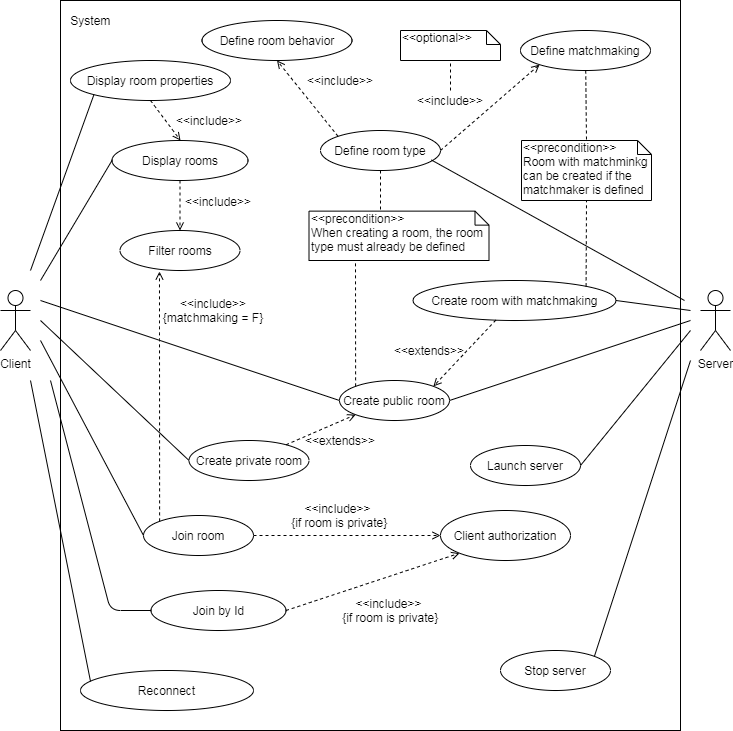
\includegraphics[scale=0.5]{images/2-scoping/system-use_cases.png}
   \centering  
   \caption{\textit{Use case diagram of the system.}}
  \label{fig:system-use_cases}
\end{figure}

\bigskip
About joined room interaction, interacting entities are client side programmer as before for clients, and, a room agent for server, intended as the server side programmer (as before) and/or the room itself with its reactive/proactive behavior defined by the programmer. 
\\
This is shown in UML use case diagram in figure \ref{fig:room-use_cases}.
\begin{figure}[H]
  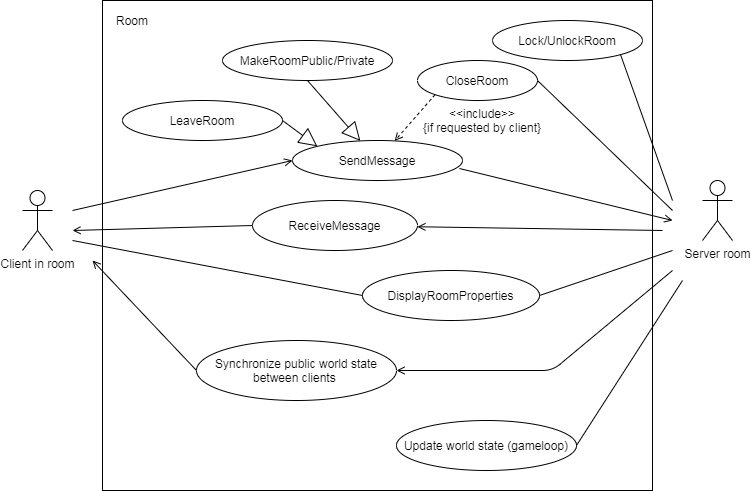
\includegraphics[scale=0.5]{images/2-scoping/room-use_cases.png}
   \centering  
   \caption{\textit{Use case diagrams of the system.}}
  \label{fig:room-use_cases}
\end{figure} 
 
 
 
 
 
 
 

 